\documentclass{template/openetcs_article}
% Use the option "nocc" if the document is not licensed under Creative Commons
%\documentclass[nocc]{template/openetcs_article}
\usepackage{lipsum,url}
\usepackage{supertabular}
\usepackage{multirow}
\usepackage{color, colortbl}
\usepackage{hyperref}
\definecolor{gray}{rgb}{0.8,0.8,0.8}
\usepackage[modulo]{lineno}
\graphicspath{{./template/}{.}{./images/}}
\begin{document}
\frontmatter
\project{openETCS}

%Please do not change anything above this line
%============================

%user specified macros
%\newenvironment{activity}[2][planned]
	{\begin{tabular}{p{0.25\textwidth}@{\hspace{0.05\textwidth}}p{0.7\textwidth}}
			\multicolumn{2}{p{\textwidth}}{\colorbox{black}{\begin{minipage}{1.1cm}\begin{center}\textsc{\footnotesize \textcolor{white}{#1}}\end{center}\end{minipage}}~~\textbf{#2}}\\
	}
	{\end{tabular}}

\newcommand{\entry}[2]{#1:&#2\\}
\newcommand{\website}[1]{Website:&\url{#1}\\}
\newcommand{\desc}[1]{\multicolumn{2}{p{\textwidth}}{#1}\\}

\newcommand{\VV}{Verification \& Validation\xspace}
\newcommand{\vv}{verification \& validation\xspace}

\newcommand{\tbd}{\colorbox{cyan}{\%\%To Be Defined\%\%}}
\newcommand{\tbc}{\colorbox{cyan}{\%\%To Be Confirmed\%\%}}
\newcommand{\todo}[1]{\colorbox{cyan}{\%\%{#1}\%\%}}
\newcommand{\nthng}[1]{}

% The document metadata is defined below

%assign a report number here
\reportnum{OETCS/WP3/D3.5.1.1}

%define your workpackage here
\wp{Work-Package 3: ``Modeling''}

%set a title here
\title{openETCS System Architecture and Design Specification}

%set a subtitle here
\subtitle{First Iteration: ETCS Kernel Functions}

%set the date of the report here
\date{September 2014}


%document approval
%define the name and affiliation of the people involved in the documents approbation here
\creatorname{Bernd Hekele}
\creatoraffil{DB-Netz}

\techassessorname{[assessor name]}
\techassessoraffil{[affiliation]}

\qualityassessorname{Izaskun de la Torre}
\qualityassessoraffil{SQS}

\approvalname{Klaus-R\"udiger Hase}
\approvalaffil{DB Netz}


%define a list of authors and their affiliation here

\author{Bernd Hekele, Peter Mahlmann, Peyman Farhangi}

\affiliation{DB-Netz AG\\
  V\"olckerstrasse 5\\
  D-80959 M\"unchen Freimann, Germany}

\author{Uwe Steinke}

\affiliation{Siemens AG}

\author{Christian Stahl}

\affiliation{TWT-GmbH}

% define the coverart
\coverart[width=350pt]{openETCS_EUPL}

%define the type of report
\reporttype{Architecture and Design Specification}


\begin{abstract}
%define an abstract here
This document gives an introduction to the architecture of the first openETCS iteration, the openETCS kernel functions. It has to be read as an add-on to the models in SysML, Scade and to additional reading referenced from the document.
\end{abstract}

%=============================
\maketitle

%Modification history
%if you do not need a modification history table for your document simply comment out the eight lines below
%=============================


\section*{Modification History}
\tablefirsthead{
\hline 
\rowcolor{gray} 
Version & Section & Modification / Description & Author \\\hline}
%\begin{supertabular}{| m{1.2cm} | m{1.2cm} | m{6.6cm} | m{4cm} |}
\begin{supertabular}{| c | c | l | l |}
0.1 & Document & Initial document providing the structure & Bernd Hekele \\\hline
0.2 & Sect.~\ref{sss:provposrep} & initial contribution and some pretty printing & Christian Stahl \\\hline
0.3 & Document & collecting feedback and completion on initial sections & Bernd Hekele \\\hline
\end{supertabular}


\tableofcontents
\listoffiguresandtables
\newpage
%=============================

%Uncomment the next line if you need line numbers for tracebility when the document is in review
%\linenumbers
%=============================


% The actual document starts below this line
%=============================


\section{Introduction}


\subsection{Motivation}
\label{sec:Motivation}

The openETCS work package WP3 aims to provide the architecture and the design of the openETCS OBU software as mainly specified in \cite{subset-026} UNISIG Subset\_026 version\_3.3.0. 

The appropriate functionality has been divided into a list of functions of different complexity (see the WP3 function list \cite{functions}).

All these functions are object of the openETCS project and have to be analysed from their requirements and subsequently modelled and implemented. With limited manpower, a reasonable selection and order of these functions is required for the practical work that allows the distribution of the workload, more openETCS participants to join and leads to an executable---limited---kernel function as soon as possible. 

While the first version of this document focuses on the first version of the limited kernel function, it is intended to grow in parallel to the growing openETCS software.


\subsection{Objectives}
\label{sec:Objectives}



The first objective of WP3 software shall be
\begin{itemize}
	\item ``Make the train run as soon as possible, with a very minimum functionality, and in the form of a rapid prototype.''
\end{itemize}
This does not contradict the openETCS goal to conform to EN50128.
\begin{itemize}
	\item After a phase of prototyping, the openETCS software shall be implemented in compliance to EN50128 for SIL4 systems.
\end{itemize}
Additional goals for this document are
\begin{itemize}
	\item Identification of the functions required for a minimum OBU kernel
	\item Architecture overview regarding the minimum OBU kernel
	\item Technical approach: Description of the proceeding and methods to be used
	\item Road map of the minimum OBU kernel functions
	\item Road map thereafter
\end{itemize}

Note: This document will be extended according to the progress of WP3. 


\subsection{History}

%-----------------------------------------------------------------------
\subsection{Goals of the openETCS Modelling Work}
%-----------------------------------------------------------------------
%\tbc
%by Uwe


\subsubsection{Functional Scope: The Minimum OBU Kernel Function}
\label{sec:FunctionalScopeTheMinimumOBUKernelFunction}

The objective ``Make the train run with a very minimum functionality'' shall be in terms of ETCS OBU translated into 
\begin{itemize}
	\item The Train moves on a track equipped with balises and determines its position.
\end{itemize}
That means, for this very first step, the train shall not supervise the maximum speed nor activate the brakes. The minimum function set shall be limited to:
\begin{itemize}
	\item Receive, filter and manage balise information received from track (see \url{https://github.com/openETCS/SRS-Analysis/issues/12})
	\item Calculate the actual train position based on balise and odometry information (see \url{https://github.com/openETCS/SRS-Analysis/issues/8})
	\item Calculate the distances between the actual train position to track elements in its front
\end{itemize}
The activities of the first iteration are collected in the \cite{firstIteration} openETCS WP3 backlog for the first iteration.

A more detailed architectural breakdown of these functions is available as a SysML model \cite{sysml-model}. Diagrams used in this document describing the architecture are taken from this model.

The design is implemented in the \cite{scade-model} Scade Model. Design documents are taken from this model. Design diagrams used in this document are generated from the model. The design documents produced from the scade model are provided in the design location on Github \cite{designFI}.

In addition, the work on this minimum functionality requires to be supported by
\begin{itemize}
	\item The availability of the ETCS language as specified in Subset UNISIG Subset\_026, chapters 7 and 8
	\item The abiltiy to link intermediate and final results with the requirements of the ETCS specification (subset\_026, \dots) 
\end{itemize}
These supporting prerequisites are under construction and therefore not completely operable actually. How to deal with these restrictions, will be outlined in chapter ???

\subsection{Glossary and Abbreviations}

\textbf{API} Application Programming Interface\\
\textbf{EVC} European Vital Computer\\
\textbf{BTM} Balise Transmission Module\\
\textbf{SRS} System Requirements Specification\\

\section{The openETCS Architecture of the initial kernel functions}

\subsection{The openETCS Tool-Chain and its impacts on the actual model}

For understanding the modelling process and the modeling guidelines, we refer to \cite{wp3-dow}. 

To summarize the design process, the following rules are in use:
\begin{itemize}
\item Papyrus / SysML is used for modelling the architecture. Functions are visible on this SysML level.
\item No behaviour model is allowed on SysML level.
\item For referencing the requirements, links from the SysML model to the requirements document (in ProR) are being used.
\item Details and especially behaviour is part of the Scade models.
\item All interfaces (see also data-dictionary below) are available on bit-level.
\item In the architecture model in SysML, all interfaces are available on a functional level for interfaces inside and outside the model and for interfaces between dedicated functions. Due to tool constrains the current model does not show all details for all interfaces (see dataDictionary).
\end{itemize}

The openETCS tool-chain for doing the modelling work consists of the following components:
\begin{itemize}
	\item [\textbf{Papyrus}]: for modelling the architecture (Kepler version).\\
	In this phase only the Kepler version of the tool can be used due to incompatibilities of the Kepler and the Luna version on the SysML model. The SysML models are stored in the following location: \url{https://github.com/openETCS/modeling/tree/master/model/sysml}.
	\item [\textbf{ProR}]: for keeping the requirements (REQIF).\\
	The subset 26 is converted into a REQIF-format and also stored in the modeling repository on Github. The openETCS toolchain supports the linking of SysML model parts to SRS-Requirements. These results are also part of the architecture.
	\item [\textbf{Scade}]: for designing and formalising the functions Scade version 15.2 is used.\\
	The models are stored in this location: \url{https://github.com/openETCS/modeling/tree/master/model/Scade}.
	With the component Scade System Scade also has a component for designing the architecture.
\end{itemize}

In principle, the synchronisation mechanism of Scade was planned to be used for synchronising the SysML architecture and the Scade models. The idea is to automatically synchronise the SysML types and blocks with the Scade type definitions and the Scade Operators. Unfortunately, with the current set of tools this idea cannot be realised. We will investigate other tools and models to find a solution. 

In addition, faults in the Kepler Papyrus version made it difficult for several members of the team to work on different submodels of the openETCS model. The issue will be solved when changing to the Luna version of Papyrus.



\subsection{The openETCS Architecture}

The following diagrams are taken from the SysML model \cite{sysml-model}.

\begin{figure}[h]
\centering
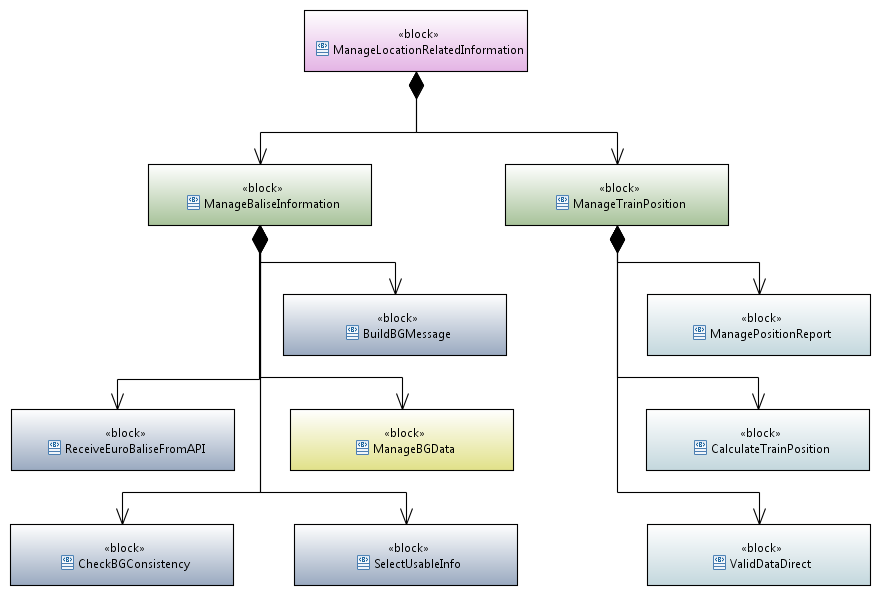
\includegraphics[scale=0.6]{../images/FunctionalArchitectureBDD.PNG}
\caption{Block Definition Diagram of the First Iteration Architecture}
\end{figure}

The diagram shows the hierarchy of the EVC model. The boundaries of the model are given with the API (interfaces into and outside the EVC model), which actually is not part of the diagram. The runtime-system of the EVC is also seen as a part outside the model.

\begin{figure}[p]
\centering
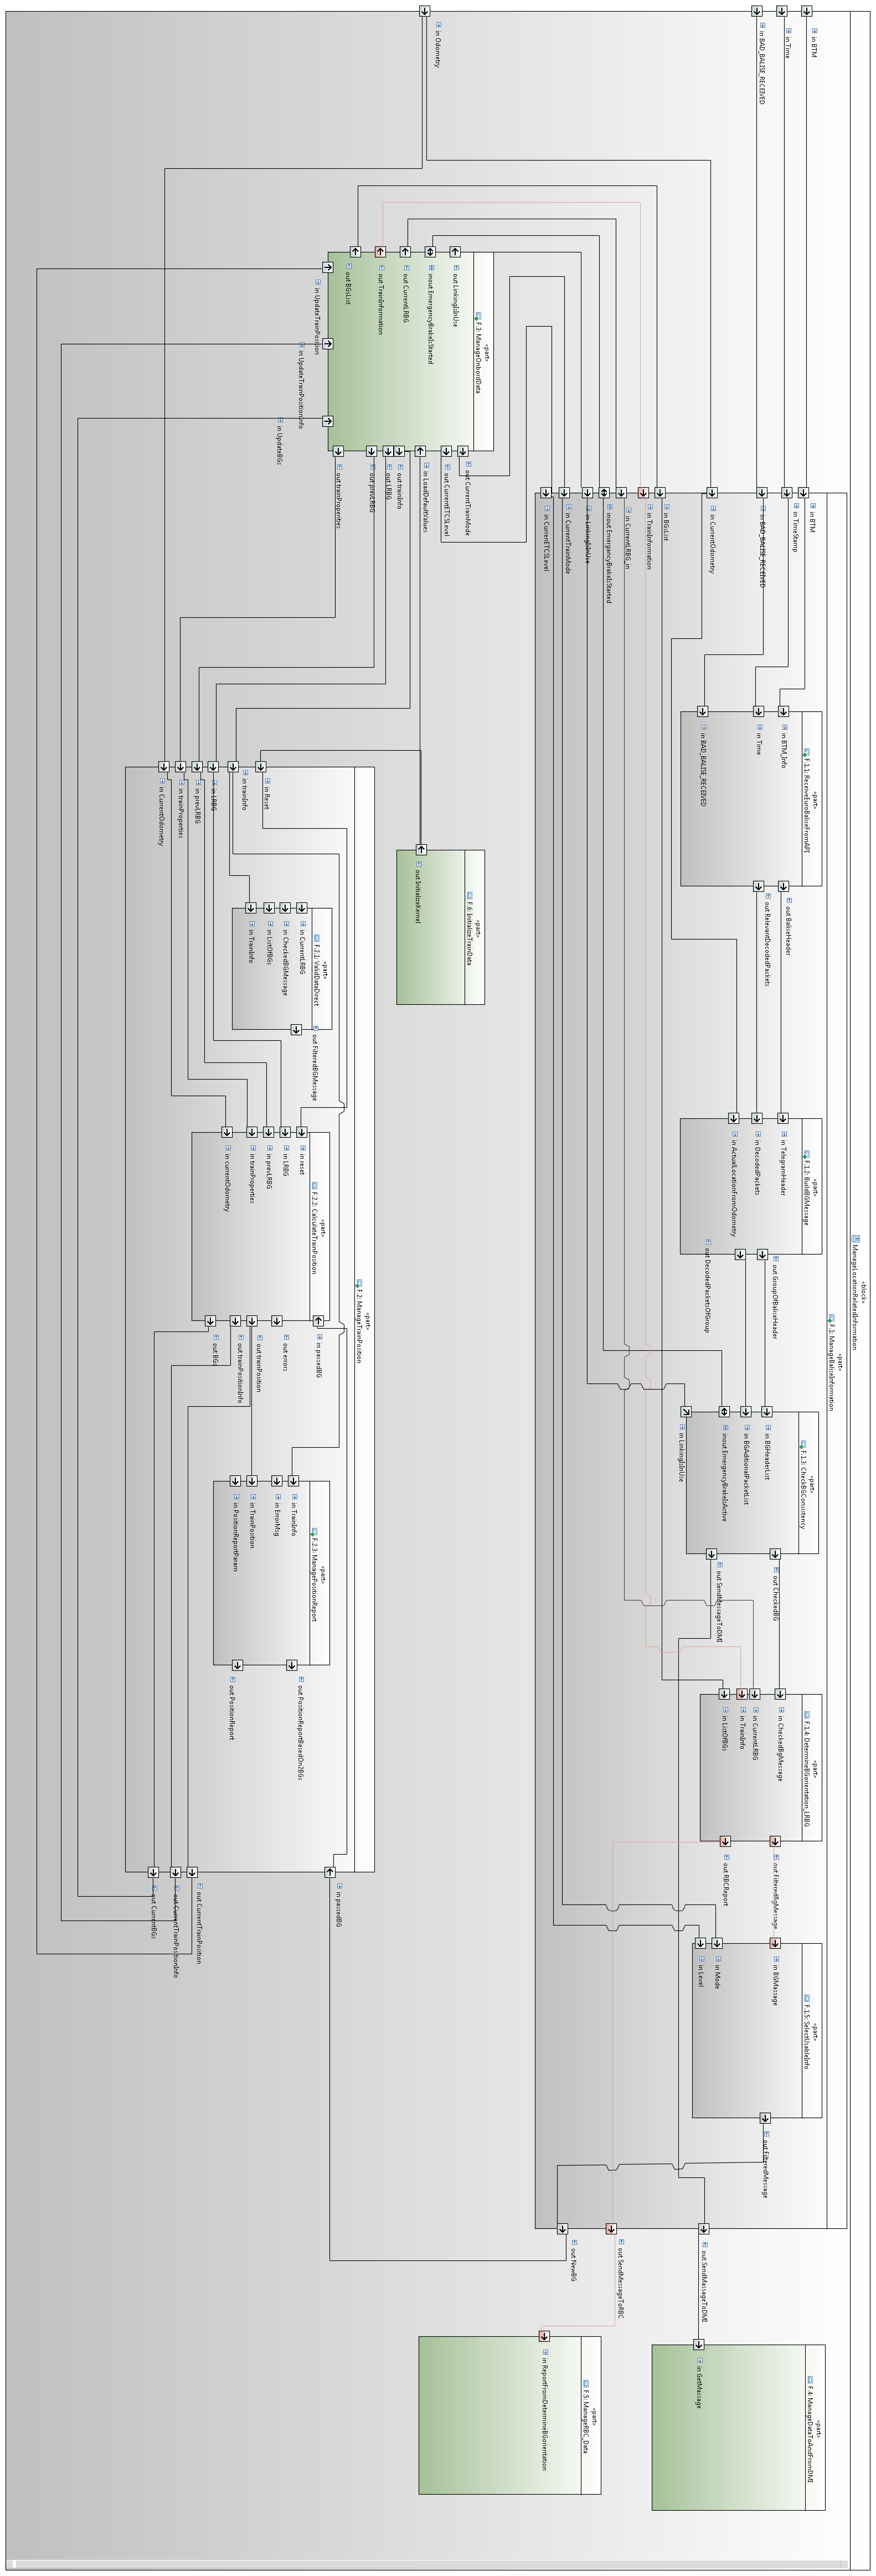
\includegraphics[scale=0.2]{../images/ManageLocationInformationIBD.PNG}
\caption{Internal Block Diagram of the First Iteration Architecture}
\end{figure}

Green blocks in this diagram are seen as data collected by the "train" without making use of the function in focus.

Input to the model is via API. The border is inside the EVC Scade model. 

\section{openETCS Functions}


\subsection{openETCS Data Dictionary}

The openETCS data Dictionary in the first iteration gives some basic constructs for the project, the definition of interfaces in a central place and the definition of the ETCS language \cite{dataDictionary}.

\subsubsection{ETCS Language}
The typedefinitions of Subset 26 chapters 7 and 8 (called the ETCS language) are provided as SysML resp. Scade types to the openETCS model. For the SysML model the types have been generated based on tools and provided as <>package<> imported to the openETCS toolschain.

\subsubsection{openETCS Interfaces}
Interfaces used within the between submodels and interfaces from ouside and to outside the EVC kernel are defined as types in the dataDictionary.

In the Scade model  the ETCS language is available in the oETCS projects S026-7 and S026-8.

\subsubsection{dataDictionary Outlook}
In the first iteration the use of the data dictionary concept is reduced to a minimum. The full openETCS process is tailored for a bigger team to cooperate and make use of tools to collect data and generate code. 

In the scade model the types needed to build the ointerfaces between models are defined in the projects Obu\_Basic\_Types.etp, BG\_Types.etp, and TrainPosition\_Types.etp.

\subsection{openETCS Generic API}


The openETCS system contains two APIs (Application Programming
Interface):
\begin{enumerate}
\item \emph{openETCS API}: the interface specification between the
EVC platform and the openETCS application;
\item \emph{model API}: the interface between the model itself written in
SCADE and the surounding run-time. Both the SCADE model and the
run-time are making the openETCS application.
\end{enumerate}

\begin{figure}[h]
\centering
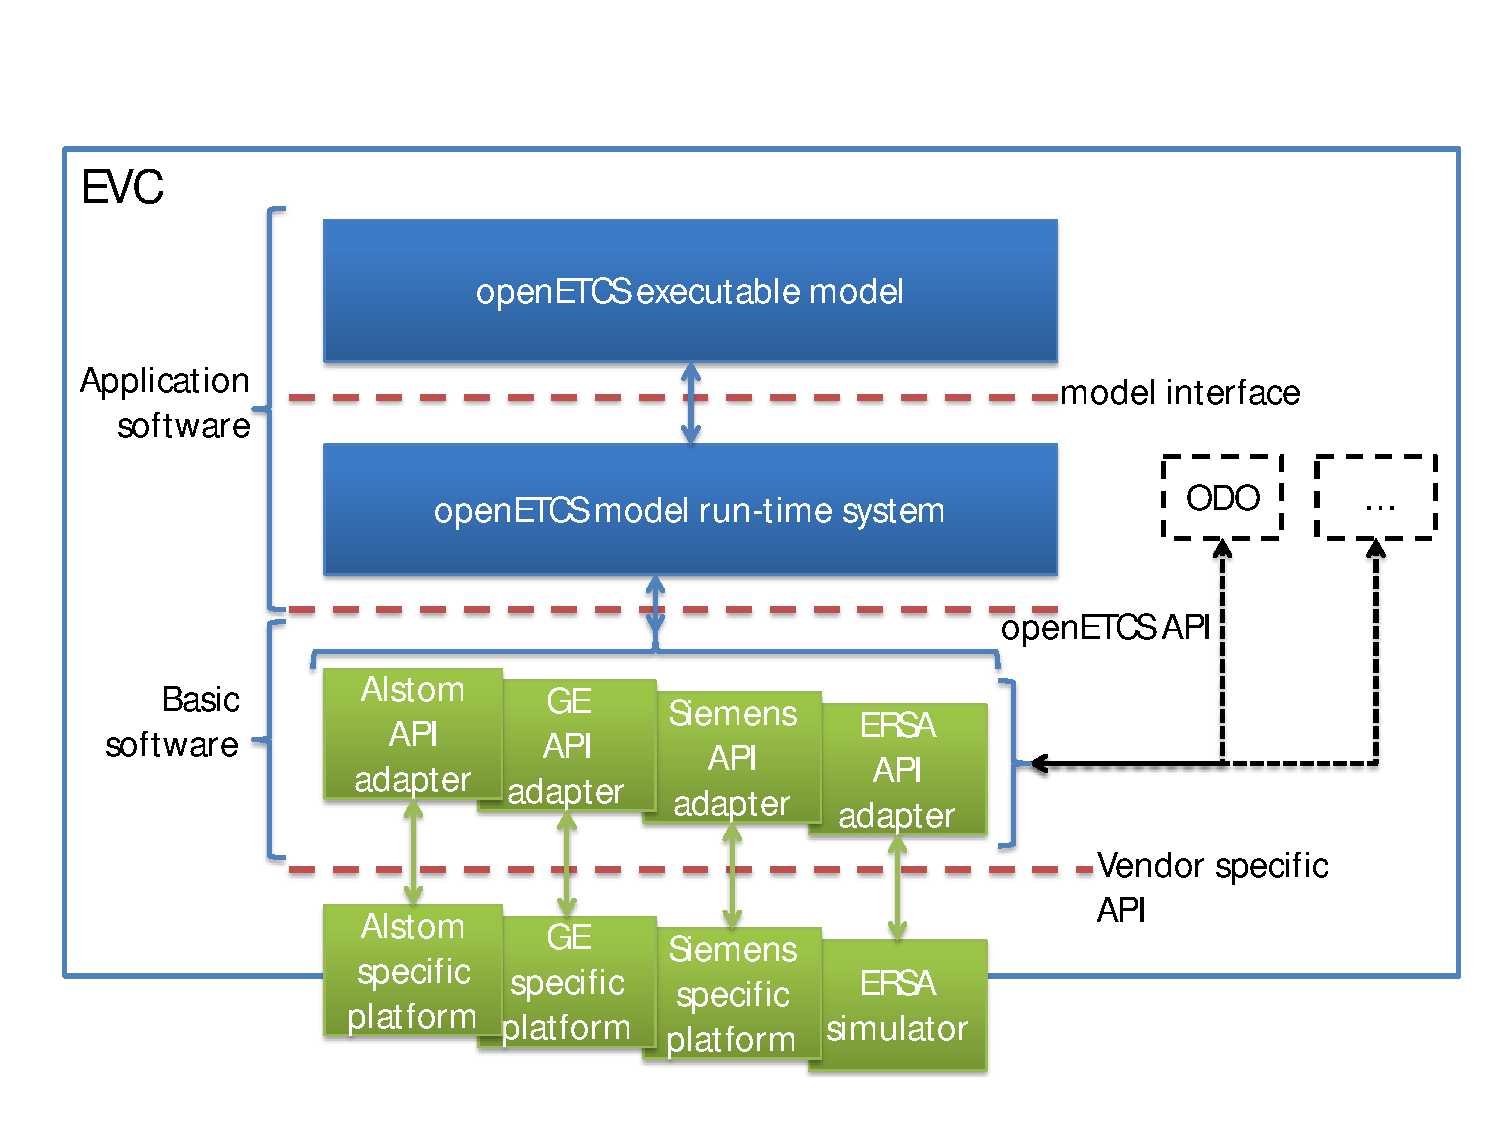
\includegraphics[width=\textwidth]{software-architecture.pdf}
\caption{openETCS software architecture}
\label{fig:software-architecture}
\end{figure}

Figure \ref{fig:software-architecture} shows both openETCS API and
model API on the software stack.

\subsubsection{openETCS API}

The openETCS API is currently defined by two documents, one written by
Alstom \cite{alstom-api} and a more abstract specification written by
openETCS members \cite{openetcs-api}.

The openETCS API defines the interfaces between the EVC platform and
the openETCS application for the following units surrounding the EVC:
\begin{itemize}
\item TIU (Train Interface Unit);
\item ODO (Odometry);
\item DMI (Driver Machine Interface);
\item STM (Specific Transmission Module, up to 8 units);
\item BTM (Balise Transmission Module);
\item LTM (Loop Transmission Module);
\item EURORADIO;
\item JRU (Juridical Recording Unit);
\item Zero or more Vendor specific unit.
\end{itemize}


\subsubsection{Model API}

The model API is currently defined by the inputs and outputs of the SCADE model.

\FIXME{How to give a precise pointer within the SCADE model? Reference
to a specific block within the model?}

For the proper working of the SCADE model, a set of assumptions are assumed:
\begin{itemize}
\item \textbf{Eurobalise (BTM)}: It is assumed that at most one
``telegram'' is provided per call of the SCADE model. This
``telegram'' is the merge of the telegrams of the balises making a
balise group.
\end{itemize}

% LocalWords:  SCADE API openETCS Alstom EVC EURORADIO Odometry balises balise


\subsection{F.1 Manage Balise Information}


\subsubsection{F.1.1 Receive Eurobalise From API}

\begin{figure}[hbtp]
\centering
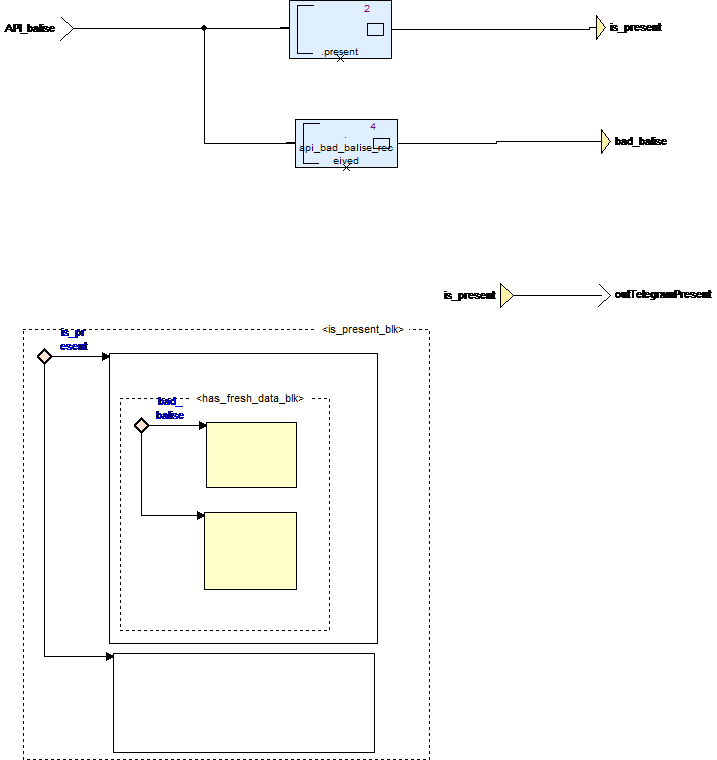
\includegraphics[scale=0.5]{../images/ReceiveEuroBaliseFromAPI_diagram.png}
\caption{Structure of ReceiveEuroBaliseFromAPI}
\end{figure}

\begin{itemize}
\item \textbf{Short Description of Functionality}\\
This function defines the interface of the OBU model to the openETCS generic API for Eurobalise Messages. On the interface, either a valid telegram is provided or a telegram is indicated which could not be received correct when passing the balise. The function passes the telegram without major changes of the information to the next entity for collecting the balise group information.
	
%\item \textbf{{Reference to the SRS (or other requirements}\\
\item \textbf{Design Constrains and Choices}\\
\begin{enumerate}
\item Decoding of balises is done at the API. Also, packets received via the interface are already transformed into a usable shape.
\item Only packets used inside the current model are passed via the interface:\\
Packet 5: Linking Information.\\
Linking Information is filled into the linking array starting from index 0 without gaps. Used elements are marked as valid. Elements are sorted according to the order given by the telegram sequence.
\end{enumerate}
\end{itemize}


\subsubsection{F.1.2 Build BG Group Message}

\begin{figure}[hbtp]
\centering
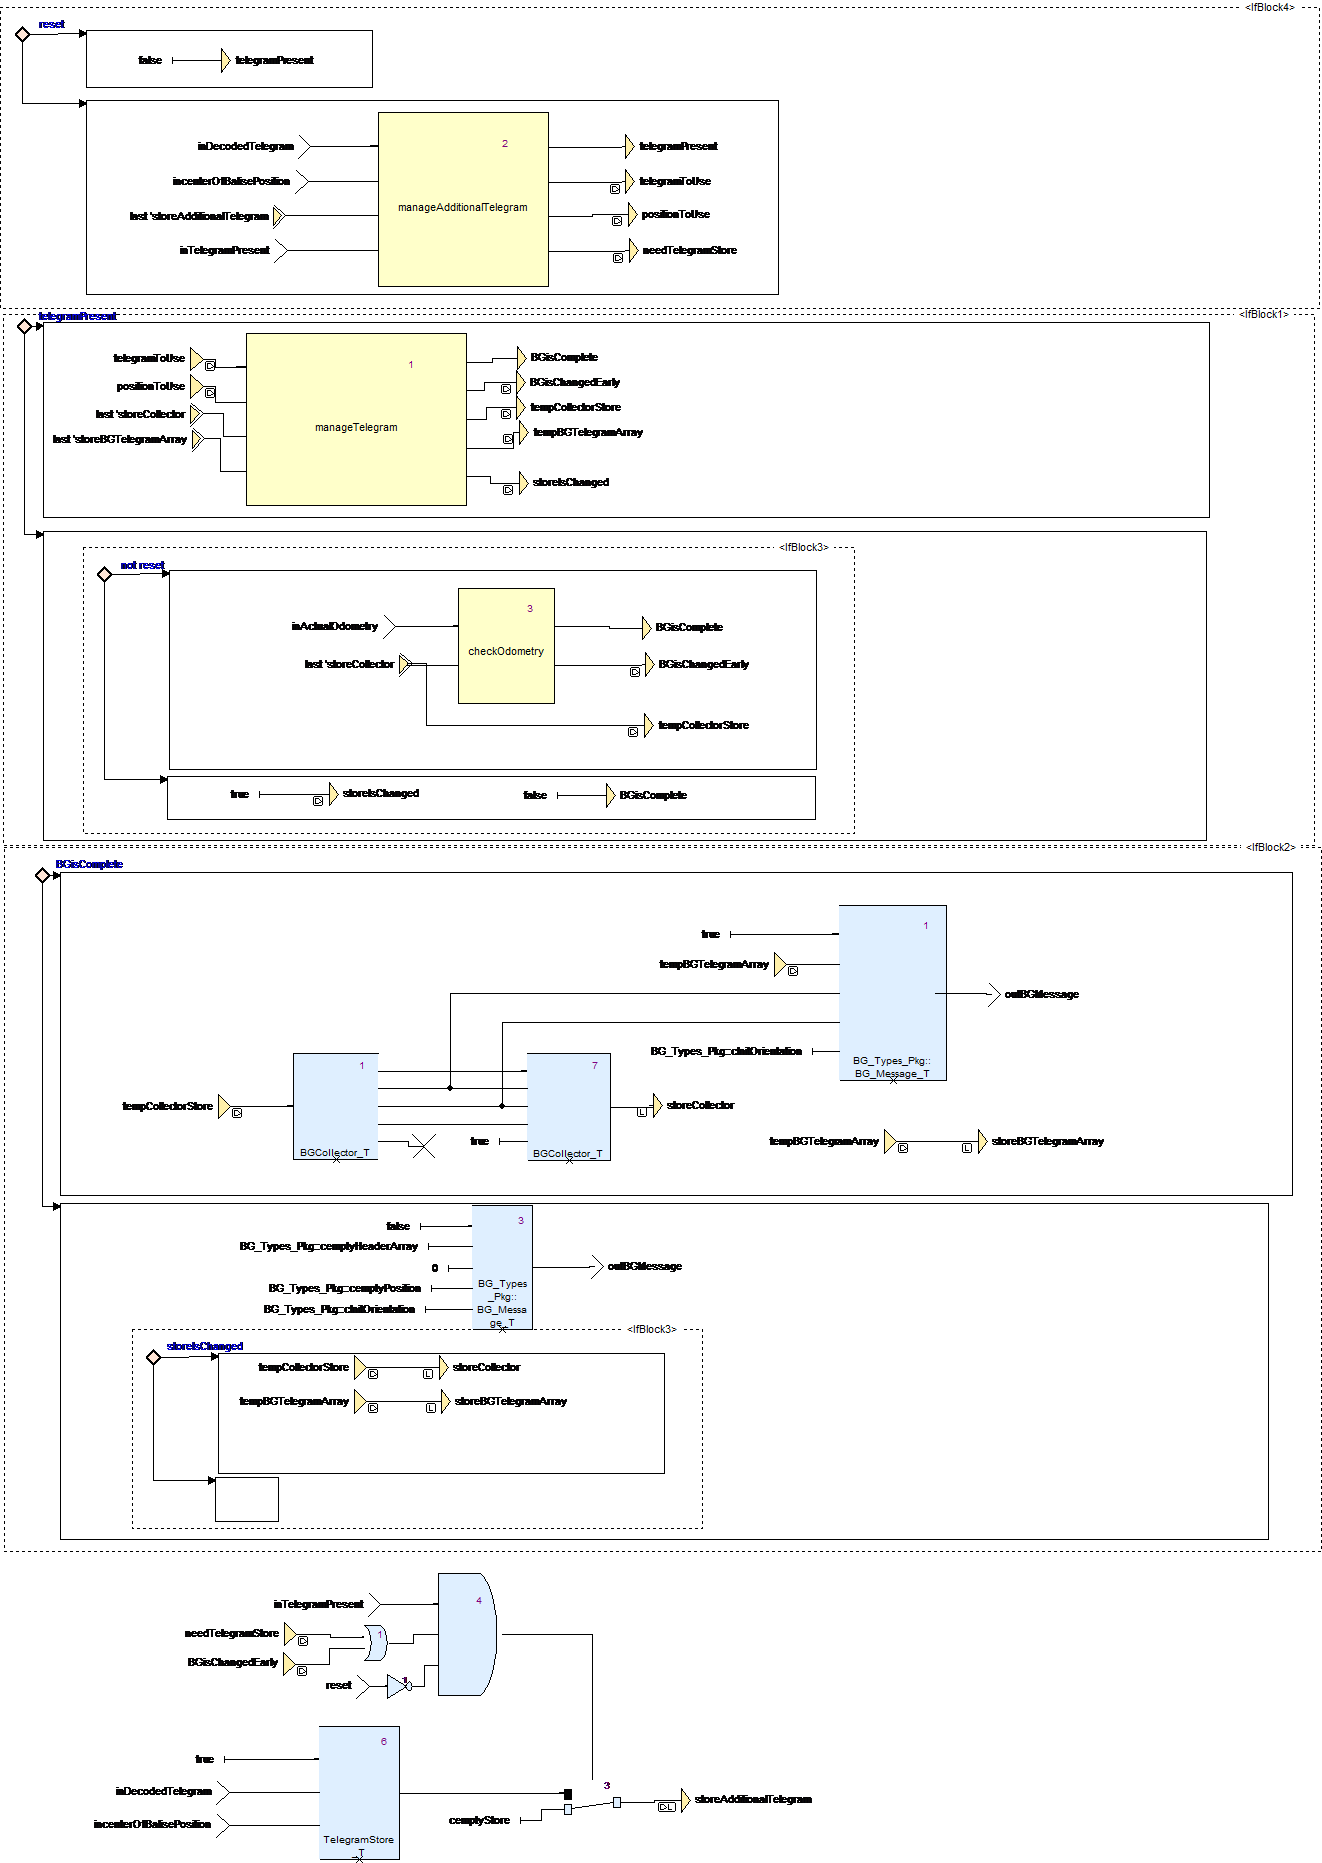
\includegraphics[scale=0.5]{../images/BuildBGMessage_diagram.png}
\caption{Structure of BuildBGMessage}
\end{figure}

\begin{itemize}
	\item \textbf{Short Description of Functionality}\\
	This entity collects telegrams received via the interface into Balise Group Information.
	\item \textbf{Reference to the SRS (or other requirements}\\
	\item \textbf{Design Constrains and Choices}\\
	\begin{enumerate}
		\item Telegrams received as invalid are passed to the ``Check-Function'' in order to process errors in communication with the trackside according to the requirements and in a single place.
		Telegrams are filled into the telegram array starting from index 0 without gaps. Used elements are marked as valid. Elements are stored according to the order given by the telegram sequence.
\item This function does not process information from the packets. The information is passed forward to the check without furhter processing of the values. 
	\end{enumerate}
\end{itemize}

\subsubsection{F.1.3 Check BG Consistency}

\begin{itemize}
\item \textbf{Short Description of Functionality}\\


%\begin{enumerate}
%\item Only packets used inside the current model are passed via the interface:\\
%Packet 5: Linking Information.\\
%\item In this function packets past with the telegrams is accumulated into a balise group information.\\
%\item Further assumption on packet 5 (based on SRS subset 26, section 8.4.1.4)\\
%(In this statement the term ``message'' is ambiguous since it can reflect to a telegram or a balise group message)
%Linking Information can only be passed once. This means, if linking information for the balise group is already collected with one of the earlier telegrams, the information will not be accumulated but overwritten.\\
%\end{enumerate}
\end{itemize}

\subsubsection{F.1.4 Determine BG- Orientation and LRBG}
\begin{itemize}
	\item \textbf{Short Description of Functionality}\\
	\item \textbf{Reference to the SRS (or other requirements}\\
	\item \textbf{Design Constrains and Choices}\\
\end{itemize}

\subsubsection{F.1.5 Select Usable Info}


\subsection{F.2 Manage Train Position}

\subsubsection{F.2.1 Validate Data Direct}
\begin{itemize}
	\item \textbf{Short Description of Functionality}\\
	\item \textbf{Reference to the SRS (or other requirements}\\
	\item \textbf{Design Constrains and Choices}\\
\end{itemize}

\subsubsection{F.2.2 Calculate Train Position}\label{sss:calctrainpos}

\begin{itemize}
\item \textbf{Short Description of Functionality}\\
The main purpose of the function is to calculate the locations of linked and unlinked balise groups (BGs) and the current train position while the train is running along the track. 

\begin{figure}[hbtp]
\centering
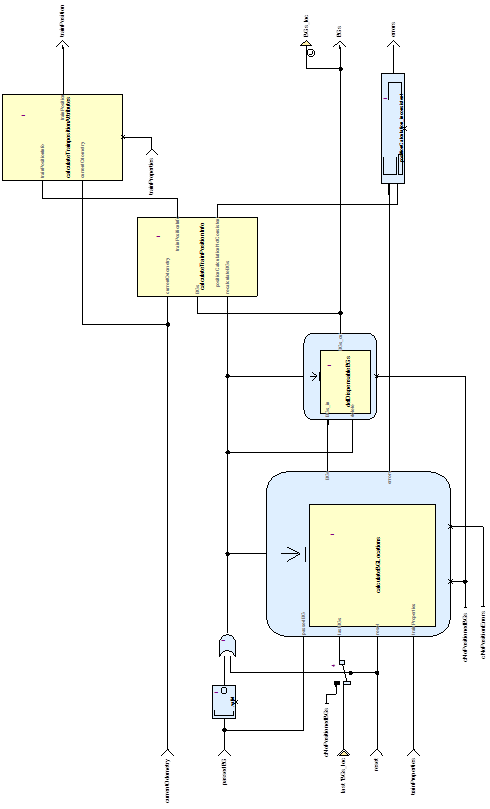
\includegraphics[scale=1]{../images/CalculateTrainPosition.png}
\caption{Structure of calculateTrainPosition}
\end{figure}


\paragraph{Functional Structure in Stages}
The whole function calculateTrainPosition is subdivided into the following steps, which are performed sequentially: 
\begin{enumerate}
\item \textbf{\textit{calculateBGLocations}}: Calculate the balise group locations\\
The first stage is triggered each time the train passes a balise group (input \textit{passedBG}). It takes the balise group header with the BG identification, the linking information (Subset 26, packet 5) and the current odometry values as inputs and calculates the location of the the passed balise group. If the passed BG has been announced via linking information previously, it takes into account the linking as well as the odometry information. If the passed BG does not meet the tolerance window announced by linking, an error flag is set. If the passed BG is an unlinked BG, its location is determined by odometry only, but related to the next previously passed linked BG, if there is one.\\
Then, if the passed BG is a linked BG comprising linking information for BGs ahead, the linking information is evaluated by creating the announced BGs and computing their locations from the linking distances.\\
The passed and the announced BGs are stored in a list \textit{BGs}, ordered by their nominal location on the track.\\
Afterwards the locations of all BGs are further improved by re-adjusting their locations with reference to the just passed BG. This optimizes the BG location inaccuries around the current train position (= location of the passed BG). 

\item \textbf{\textit{delDispensableBGs}}: Delete dispensable balise groups\\
The second stage removes balise groups supposed not to be needed any longer from the list of \textit{BGs}.\\
If the number of stored passed linked BGs exceeds the maximum number of eight as specified in subset-26-3.6.2.2.2 c), all BGs astern are deleted.
If only (passed) unlinked BGs are in the list and exceed the number of \textit{cNoOfAtLeast\_x\_unlinkedBGs}, all passed BGs astern to those are removed from the list. 

\item \textbf{\textit{calculateTrainPositionInfo}}: Calculate train position information.\\
This stage take the list of stored BGs and the current odometry values as inputs and steadily provides the current train position. 

\item \textbf{\textit{calculateTrainpositionAttributes}}: Calculate train position attribute information.\\
This stage provides several additional position related attributes that might conveniently be used by subsequent consumers in the architecture. It requires the actual LRBG and the previous LRBG to be assigned external from the list \textit{BGs}. 

\end{enumerate}

\item \textbf{Reference to the SRS (or other requirements)}\\
\\
The component calculateTrainPosition determines the location of linked and unlinked balise groups and the current train position during the train trip as specified mainly in subset-026-3.6

\item \textbf{Design Constraints and Choices}\\
\\
The following constraints and prerequisites apply:

\begin{enumerate}
\item The input data received from the balises groups must have been checked and filtered for validity, consistency and the appropriate train orientation before delivering them to calculateTrainPosition. 
\item The storage capacity for balise groups is finite. calculateTrainPosition will raise an error flag when a balise group cannot be stored due to capacity limitations.
\item calculateTrainPosition will raise an error flag if a just passed balise group is not found where announced by linking information. It will not (yet) detect when an announced balise group is missing. 
\item calculateTrainPosition is not yet prepared for train movement direction changes. 
\item calculateTrainPosition does not yet consider repositioning information.
\end{enumerate}

\end{itemize}

\subsubsection{Provide Position Report}\label{sss:provposrep}

\begin{figure}[ht]
\centering
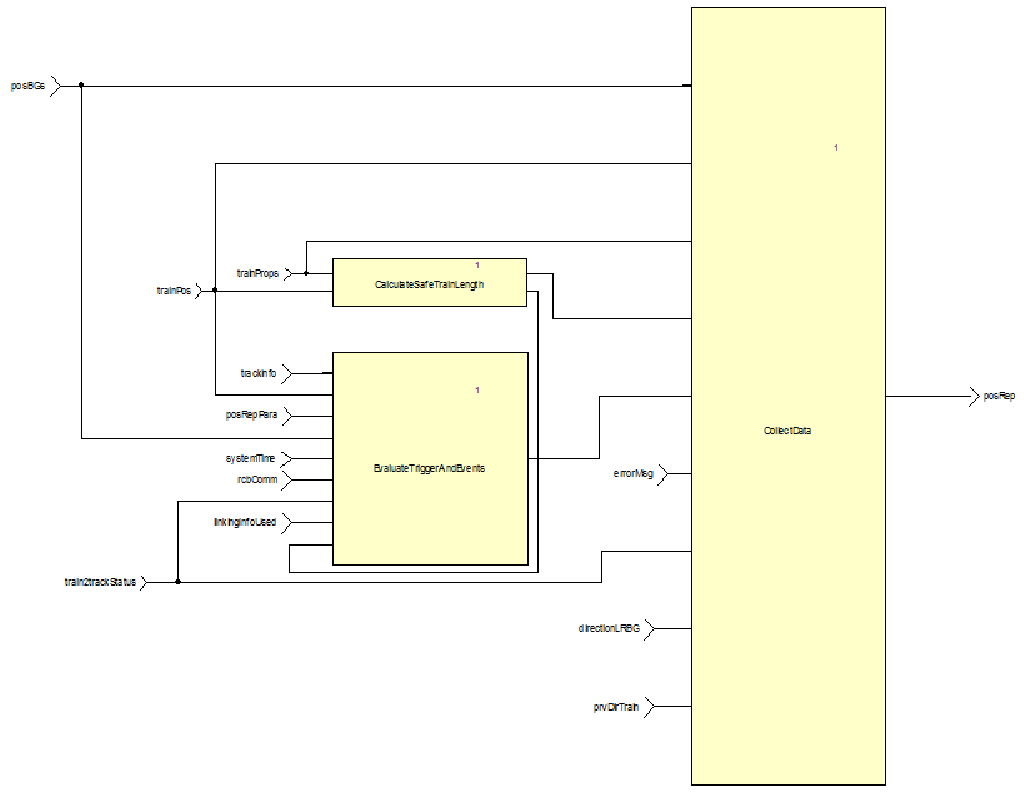
\includegraphics[scale=0.6]{../images/ProvidePositionReport.pdf}
\caption{Structure of component ProvidePositionReport}\label{fig:provideposrep}
\end{figure}

\begin{itemize}
\item \textbf{Short Description of Functionality}\\
This function takes the current train position and generates a position report which is sent to the RBC. The point in time when such a report is sent is determined from event, on the one hand, and position report parameters---which are basically triggers---provided by the RBC or a balise group passed, on the other hand. The functionality is modeled using three operations, as shown in Fig.~\ref{fig:provideposrep}, which are explained below.
\begin{description}
	\item[CalculateSafeTrainLength] Calculates the the safeTrainLength according to Chapt.~3.6.5.2.4/5.
\verb+safeTrainLength = absolute(EstimatedFrontEndPosition - MinSafeRearEnd)+, where
\verb+MinSafeRearEnd = minSafeFrontEndPosition - L_TRAIN+
	\item[EvaluateTriggerAndEvents] Returns a Boolean modeling whether the sending of the next position report is triggered or not. It is the conjunction of the evaluation of all triggers (PositionReportParameters, i.e., Packet 58) and events (see Chapt.~3.6.5.1.4).
	\item[CollectData] In this operation, data of Packet0, \dots, Packet5 and the header is aggregated to a position report.
\end{description}
\item \textbf{Reference to the SRS (or other requirements}\\
Most of the functionality is described in subset 26, chapter~3.6.5.
\item \textbf{Design Constrains and Choices}\\
\begin{enumerate}
	\item The message length (i.e., attribute \verb+L_MESSAGE+) is by default set to 0; the actual value will be set by the Bitwalker/API.
	\item The attribute \verb+Q_SCALE+ is assumed to be constant; that is, all operations using this attribute do not convert between different values of that attribute.
	\item \textit{PositionReportHeader}: The time stamp (i.e., attribute \verb+T_TRAIN+) is not set; this should be done once the message is being sent by the API
	\item \textit{Packet4}: When aggregating the data for this packet, an error message might be overwritten by a succeeding error message. Because the specification only allows to sent one error in one position report, errors are not being stored in a queue, for instance.
	\item \textit{Packet44}: This packet is currently not contained in a position report as it is not part of the kernel functions.
	\item The usage of attributes \verb+D_CYCLOC+ and \verb+T_CYCLOC+ as part of the triggers specified by the position report parameters (i.e., Packet 58 sent by the RBC) may lead to unexpected results if a big clock cycle together with small values for the attributes is used. The cause is that the current model increments at every clock cycle the reference value for the distance and time by at most \verb+D_CYCLOC+ and \verb+T_CYCLOC+, respectively and not a factor of it.
\end{enumerate}
\item \textbf{Open Issues}
\begin{enumerate}
	\item Operation \textit{EvaluateTriggerAndEvents} currently ignores parameters \verb+N_ITER+, \verb+D_LOC+ and \verb+D_LGTLOC+ which allow to specify up to 32 position at which a report has to be sent. The positions are relative to the location of a reference balise group. If the RBC sends packet 58, then it also provides a reference balise group; otherwise, if packet 58 is sent by a balise group, then this balise group serves a the reference balise group. Possible realisation in the model: Extend in the interface posRepPara (i.e., Packet 58) by a \verb+NID_BG+ referring to the reference balise group. Am assumption would be that this BG can be found in the list of passed balise group provided by \textit{CalculateTrainPosition} in Sect.~\ref{sss:calctrainpos}.
	\item The specification requires to store the last eight balise groups for which a position report has been sent (see 3.6.2.2.2.c).
	\item For all reports that contain Packet 1 (i.e., report based on two balise groups), the RBC sends a coordinate system. It is unclear where this has to be stored (i.e., somehow the balise groups have to be stored in a database which has then to be updated), see 3.4.2.3.3.6. Moreover, such a coordination system can be invalid and then has to be rejected (see 3.4.2.3.3.7-8). On a more abstract level, we need to think about the interface between the RBC and the OBU or a proper abstraction thereof.
	\item The decision whether a the report consists of packet 0 or packet 1, which is provided in 3.4.2.3.3, is currently not completely modeled. So far, 3.4.2.3.3.1 has only been modeled, thereby assuming ``the last balise group detected'' is the last balise group and not the LRBG. 3.4.2.3.3.2 is unclear. To model 3.4.2.3.3.4 I need information about the last two valid balise groups and the train running direction. This information can be obtained by adding a memory or this information will be provided by \textit{CalculateTrainPosition} in Sect.~\ref{sss:calctrainpos}. Likewise, also 3.4.2.3.3.5 requires knowledge about the last two valid balise groups.
\end{enumerate}
\end{itemize}



%\nocite{*}
\bibliographystyle{unsrt}
%\bibliographystyle{plain}
%\bibliographystyle{alpha}
%\bibliographystyle{annotate}
%\bibliographystyle{klunamed}
\bibliography{architecture}


%===================================================
%Do NOT change anything below this line

\end{document}
